% For plaintext use only
\documentclass{article}

\usepackage{xltxtra}
\usepackage{amsmath}
\usepackage{tikz}
\usepackage{unicode-math}
\usepackage{fontspec}
\setmathfont{xits-math.otf}

\tikzset{node distance=2cm, auto}

\author{Víctor López Juan}
\title{Chapter 1}

\begin{document}

\begin{enumerate}
  \item[7.]

    Sets/2 has, as objects, arrows (X → 2), and, has
    an arrow $\bar{f} : α : (A → 2) → β : (B → 2)$

    iff there is an arrow f in set , $f : A → B$, for which the following
    diagram commutes:

    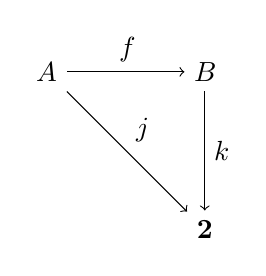
\begin{tikzpicture}
      \node (A) {$A$};
      \node (B) [right of=A] {$B$};
      \node (2) [below of=B] {$\text{\bf 2}$};
      \draw[->] (A) to node {$f$} (B);
      \draw[->] (A) to node {$j$} (2);
      \draw[->] (B) to node {$k$} (2);
    \end{tikzpicture}

    \begin{equation}
    \begin{array}{rll}
      F : & Sets/2           & → Sets × Sets              \\
          & α : (X → 2)      & → α^{-1}(a) × α^{-1}(b)      \\
          & \bar{f} : α → β  & → <f|α^{-1}(a), f|α^{-1}(b)>  \\
    \end{array}
    \end{equation}

    The function is well defined because, for every $\bar{f} : α → β$,
    $α = b ◦ f$, which means that, for $* = a,b$, if
    $x ∈ α^{-1}(*)$, then $f(x) ∈ β^{-1}(*)$.

    This is a functor:

    $F(id_{A→2}) = id_{α^{-1}(a)×α^{-1}(b)}$

    And, if $\bar{g} : α → β$, $\bar{f} : β → γ$
    \begin{equation}
    \begin{array}{rcl}
       & F(\bar{f} ◦ \bar{g})                        & = \\
    =  & <(f ◦ g)|α^{-1}(a), (f ◦ g)|α^{-1}(b)>        & = \\
    =  & <(f|β^{-1}(a) ◦ g|α^{-1}(a), f|β^{-1}(b) ◦ g|α^{-1}(b)> & = \\
    =  & F(\bar{f}) ◦ F(\bar{g}) & \\ 
    \end{array}
    \end{equation}

    It's not an isomorphism, as:

    Assume that $F^{-1}$ exists.

    Then $F(F^{-1}({a} × {a})) = {a} × {a}$.

    However, this can't be the case: pairs of sets in the image
    of $F$ are always disjoint.

    Now:

    \begin{equation}
    \begin{array}{rll}
      F : & Sets/1           & → Sets                   \\
          & α : (A → 1)      & → α^{-1}(a)   = A         \\
          & \bar{f} : α → β  & → f|α^{-1}(a) = f|A  = f  \\
    \end{array}
    \end{equation}

    It is a functor, as it clearly respects identity and composition.

    \begin{itemize}
      \item 1 is a terminal object. Therefore, for every object X,
        including itself, there is a unique arrow $X → 1$.
      \item For every arrow $f : A → B$ in Sets,the following diagram
        commutes:
        
  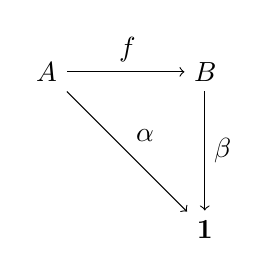
\begin{tikzpicture}
      
      \node (A) {$A$};
      \node (B) [right of=A] {$B$};
      \node (1) [below of=B] {$\text{\bf 1}$};
      \draw[->] (A) to node {$f$} (B);
      \draw[->] (A) to node {$α$} (1);
      \draw[->] (B) to node {$β$} (1);

  \end{tikzpicture}

     There's a unique arrow $α : A → 1$, so, if $f ◦ β : A → 1$,
     $f ◦ β = α$.

    \end{itemize}

    Therefore, the functor G is well defined:

    \begin{equation}
    \begin{array}{rll}
      G : & Sets             & → Sets/1         \\
          & A                & α : A ↦ 1  \\
          & f : A → B        & \bar{f} : α → β  \\
    \end{array}
    \end{equation}

    And is an inverse for F:

    $F ◦ G = G ◦ F = id$,

    which means that F is an isomorphism, and G is it's inverse
    
  \item[12.]

    Errata: The universal property is $U(\bar{h}) ◦ i = f$.

    The book defines graphs as multigraphs (parallel edges are allowed). The 

    \begin{equation}
    \begin{array}{rll}
    U : & Cat         & → Graph            \\
        & (O, A)      & ↦ (O, A, dom, cod) \\
        & F : C₁ → C₂ & ↦
            \begin{array}{rll}
              μ : & U(C₁)       & → U(C₂)                 \\
                  &  V          & ↦ F(V)                  \\
                  & a           & ↦ F(a) \\ 
            \end{array}
            \\
    \end{array}
    \end{equation}
    
    \begin{description}
      \item[Existence]

        \begin{equation}
          \begin{array}{rll}
            \bar{h} : & C(G)    & → D                                     \\
                      & \bar{h}(v)                & ↦  f(v)               \\                
                      & \bar{h}(id_V)             & ↦  id_{f(v)}            \\                
                      & \bar{h}(e_1 ◦ … ◦ e_n)    & ↦  f(e₁) ◦ … f(e_n)    \\                
          \end{array}
        \end{equation}

        $\bar{h}$ satisfies $U(\bar{h}) ◦ i = f$ by construction. 

      \item[Uniqueness]

        
        Assume $λ$ such that $U(λ) ◦ i = f$, $λ  : C(G) → D$ a functor.

        Then:
        For every vertex v is a vertex, then:

        \begin{equation}
          \begin{array}{rcl}
               & λ(v)       & = \\
             = & U(λ)(v)    & = \\   % definition of U
             = & U(λ)(i(v)) & = \\ % definition of i
             = & f(v)       & = \\  % hypothesis
             = & \bar{h}(v) &   \\  % definition of \bar{h}
          \end{array}
        \end{equation}
               
        $λ(id_V) = id_{λ(v)} = id_{f(v)} = \bar{h}(id_V)$

        λ is a functor, so:

        \begin{equation}
          \begin{array}{rcl}
             & λ(e_1 ◦ … ◦ e_n)          & = \\
           = & λ(e_1) ◦ … ◦ λ(e_n)       & = \\  % λ is a functor
           = & U(λ)(e_1) ◦ … ◦ U(λ)(e_n) & = \\  % definition of U
           = & f(e_1) ◦ … ◦ f(e_n)       & = \\  % hypothesis
           = & \bar{h}(e_1 ◦ … ◦ e_n)    &   \\
          \end{array}
        \end{equation}
    \end{description}

\end{enumerate}


\end{document}
  
